\documentclass[paper=a4, fontsize=11pt]{scrartcl}
\usepackage[T1]{fontenc}
\usepackage{fourier}

\usepackage[margin=1in]{geometry}
\setlength{\parskip}{0.5em}

\usepackage[english]{babel}
\usepackage[protrusion=true,expansion=true]{microtype}	
\usepackage{amsmath,amsfonts,amsthm} % Math packages
\usepackage[pdftex]{graphicx}	
\usepackage{url}

% cref command
\usepackage[noabbrev,capitalise]{cleveref}

%%% Custom sectioning
\usepackage{sectsty}
\allsectionsfont{\centering \normalfont\scshape}

%%% Custom headers/footers (fancyhdr package)
\usepackage{fancyhdr}
\pagestyle{fancyplain}
\fancyhead{}											% No page header
\fancyfoot[L]{}											% Empty 
\fancyfoot[C]{}											% Empty
\fancyfoot[R]{\thepage}									% Pagenumbering
\renewcommand{\headrulewidth}{0pt}			% Remove header underlines
\renewcommand{\footrulewidth}{0pt}				% Remove footer underlines
\setlength{\headheight}{13.6pt}

%%% Equation and float numbering
\numberwithin{equation}{section}		% Equationnumbering: section.eq#
\numberwithin{figure}{section}			% Figurenumbering: section.fig#
\numberwithin{table}{section}				% Tablenumbering: section.tab#

%%% Maketitle metadata
\newcommand{\horrule}[1]{\rule{\linewidth}{#1}} 	% Horizontal rule

\title{
    \normalfont
    \large \textsc{University of Groningen \\ Web and Cloud Computing} \\ [22pt]
    \horrule{0.5pt} \\[0.4cm]
    \huge Docker Dashboard \\ Project Report \\
    \horrule{0.5pt} \\[0.5cm]
}

\usepackage{array}

\author{%
	\begin{tabular}{c}
    	Davide Pedranz \\
        \small d.pedranz@student.rug.nl \\
        \small S3543757
    \end{tabular}
    \and
    \begin{tabular}{c}
    	Yuying Andrew Chen \\
        \small y.chen.66@student.rug.nl \\
        \small S3421902
    \end{tabular}
    \and
    \begin{tabular}{c} 
    	Francesco Segala \\ 
    	\small f.segala@student.rug.nl \\
        \small S3521885
    \end{tabular}
}

\date{\vspace{.5cm} \normalsize\today}

\begin{document}
    \maketitle
    
    \tableofcontents
    \pagebreak

    \section{Introduction}
\label{sec:introduction}

In this project, we developed a web-application to manage a Docker Swarm cluster. The application is designed to be scalable, fault-tolerant, and easy to deploy and manage.
It allows user to visualize the running services, create new services, modify or delete the running ones, and visualize the real-time events happening in the cluster.
Besides, the access to the application is restricted to only authenticated and authorized users. Thus, only the administrator is able to assign and revoke permissions to the users. 

\cref{sec:architecture} describes the general architecture of the application, the functionalities provided by each component, the strategies adopted to resist failures and the most important design choices.
\cref{sec:deployment} discusses how the application is deployed in order to be fault-tolerant from the point of view of the infrastructure (e.g. resist the crash of an entire virtual machine in the cluster).
\cref{sec:conclusions} summarizes the work accomplished, the achieved results and possible improvements or future developments for the application.

    \section{Architecture}
\label{sec:architecture}

\begin{figure}[h]
	\centering
	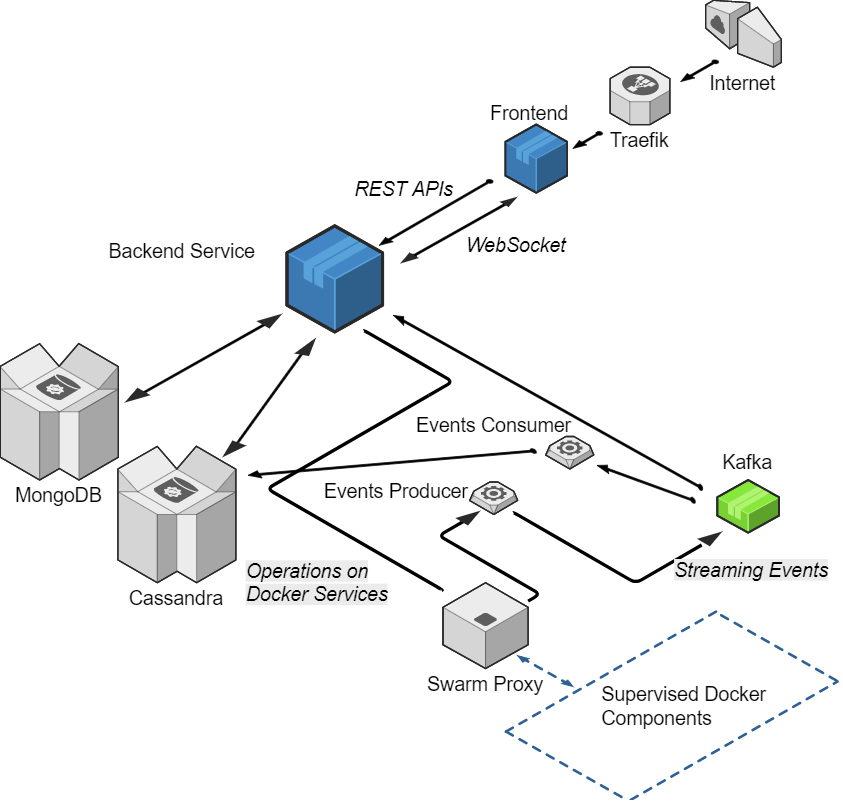
\includegraphics[width=0.92\columnwidth]{architecture}
	\caption{Architecture of the application.}
	\label{fig:architecture}
\end{figure}

\cref{fig:architecture} shows the architecture of the application.
First, all the incoming requests are handled by Traefik (load balancing), and then assigned to frontend. The frontend uses REST APIs and WebSockets to interact with the backend. 
The backend is also able to manipulate the components of Docker Swarm through the Docker Swarm proxy.
All data related to the users is saved to MongoDB, the Swarm events are saved in Cassandra.
Kafka is used as a message queue to support the events' streaming.
All details are described in next subsections.

All component in the application are packaged in Docker\footnote{\url{https://www.docker.com/}} containers.
We will discuss in detail how the application is deployed in \cref{sec:deployment}.

\subsection{Reverse Proxy}
All external incoming requests are handled through Traefik\footnote{\url{https://traefik.io/}}, a level 7 fast reverse proxy and load balancer.
Traefik forwards the requests for the frontend and the backend, depending on the requested path.
It uses a round-robin strategy to achieve load-balancing between the available instances of the services.

Traefik is configured to automatically retrieve the services running in the cluster using the Docker Swarm APIs.
This allows to set up the correct routes automatically based on the labels specified for each service at deployment time.
It also allows Traefik to read the status of each instance and forward requests only to the healthy ones.

As a bonus point, Traefik supports HTTPS protocol to protect all incoming connections.
It uses the Let's Encrypt\footnote{\url{https://letsencrypt.org/}} to automatically setup and renew the needed SSL/TLS certificates.
In our setup, Traefik redirects all HTTP requests to HTTPS, terminates the TLS connections and enables.
If the client supports it, Traefik will automatically upgrade to HTTP/2 for better performances.


\subsection{Frontend}
The frontend is a single page application written in Typescript using Angular 4\footnote{\url{https://angular.io/}} and ngrx (Reactive Extensions for Angular)\footnote{\url{https://ngrx.github.io/}}.
The user interface is implemented using Angular Material\footnote{\url{https://material.angular.io/}} and Angular Flex\footnote{\url{https://github.com/angular/flex-layout}}.
The code is organized in modules (services, events, users, etc.);
in each module, the user interface is implemented as a set of independent components, combined together to render the final page.
We followed the Angular official style guide\footnote{\url{https://angular.io/guide/styleguide}}.

\paragraph{ngrx}
The most interesting part about the frontend is the use of ngrx.
The application has a single, centralized and immutable store:
the store can only be modified by a reducer, a pure function that takes as input the previous state and some action and return a new state;
all components in the frontend dispatch actions when they need to modify the store and render the UI using the store as the single truth source.
The store is accessed using the observable pattern:
this allows to completely drop the traditional 2-way data-binding used in many MVC frameworks, since the views are only updated when the store changes, and brings much better performances since the framework does not need to poll for changes.
When actions require some side-effects (i.e. they can not be handled with a pure function, for example an HTTP call), we use ngrx effects:
the effects are triggered by some actions, which usually have side effects (HTTP calls, connect to a WebSocket, etc.) and produce new actions when the side-effects terminates.
For more information about this technology, please refer to the official ngrx documentation.

We will give an example of how this paradigm applies to our frontend.
To access the dashboard, the user needs to login.
The first time the user opens a page, the Angular Router uses the information from the store to determine if the user is authenticated or not.
Assuming the user is not authenticated, the router will then redirect user to the login page.
Once the user inserts its credentials and press the button ``login'', the associated controller dispatches an action ``login'', from when the reducer changes the store, so the view will be automatically updated to show a loading bar.
At the same time, an effect is triggered. This will perform the HTTP call to the backend.
Once the HTTP call is terminated (either with a success or an error), the effect will dispatch a new action, for example ``login success''.
The reducer will change the store again, and the view will be updated and show the dashboard;
another effect is triggered and saves the token obtained from the backend in the local storage.
For another scenario that the user closes and reopens the browser,
the application will trigger a ``load token'' action and an effect will try to load the token from the local storage.
If it finds a token, it will dispatch an action ``login success'', so the application can know that the user is logged in.

This pattern seems to be quite complex, but it allows a very strong separation of concerns between the UI logic and the business logic.
It makes the application easy to test and maintain.
The UI only renders the view using the current store. When a component needs to perform some actions (e.g., login), it simply dispatches the corresponding actions, then some other pieces of the application (e.g., an effect) will handle it and update the store if needed.
Actions can be dispatched by any component, and effects can be easily replaced, since they only consume and/or produce actions.

\paragraph{Communication with the Backend}
The frontend communicates with the backend using both REST APIs and WebSockets.
The REST APIs are used to handle the login, manage the services running in the Docker Swarm cluster, and manage the users.
The WebSocket is used to stream the events happening in the cluster.

The frontend heavily relies on the backend to retrieve the needed data.
If machine or container crashes on the server, the reverse proxy needs some time to realize it and could still try to route requests to the crashed instance.
The frontend retries all HTTP request that fails with some 5xx error code (indicating something not working properly on the server) multiple times, waiting a small amount of time between each retry.
Another possible point of failure is the WebSocket.
Since it relies on a TCP connection with the backend, the WebSocket can be closed in case of any networking problem on the client side or failures on the server.
Similarly to failed HTTP requests, the frontend will automatically detect closed WebSockets and reconnect to the server after a small amount of time.

The frontend is replicated to achieve fault tolerance.
Since it is just a set of static files, no particular extra effort is needed (we simply run multiple containers with the frontend image).

\paragraph{Build}
The Angular 4 application is compiled when the Docker image is created.
We exploit a new feature of Docker called multi-stage builds\footnote{\url{https://docs.docker.com/engine/userguide/eng-image/multistage-build/}}:
the build process uses an image with Node.js pre-installed to compile the application, then only the files needed to run the application in production are copied to the final image.
In this way, we avoid copying the source and other unneeded files to the final image.
As a bonus, the developer does not need to install Node.js or any other tool but Docker to compile, package and run the frontend.
The final image uses Nginx\footnote{\url{https://nginx.org/}} to serve the compiled application.
Nginx is configured to use gzip to compress the pages for the client and uses a strict Content-Security-Policy\footnote{\url{https://developer.mozilla.org/en-US/docs/Web/HTTP/CSP}} for greater security against XSS and other attacks.


\subsection{Backend}
The backend is written in Scala using the Play Framework\footnote{\url{https://www.playframework.com/}}.
It handles authentication, authorization, and access to resources such as users, services running in Docker Swarm and Docker events.
The entire backend is asynchronous to scale to very high loads with limited resources.

There is a clear separation of concerns in our implementation.
Authentication and authorization are handled outside the controllers (described later in detail).
Each entity is represented with a Scala \texttt{case class}.
Access to the databases is implemented in separate classes.
Calls to the Docker Swarm APIs are isolated in one class.
The controllers only need to validate the requests, add some business logic (e.g., a user cannot delete itself) and invoke the repository / services classes to perform the low-level operations.
We use the build-in dependencies injector to wire-up together all the pieces.

Dependency injection also facilitate the testing, since it is possible to mock some parts of the application and test one specific functionality in isolation.
We wrote unit test cases using ScalaTest\footnote{\url{http://www.scalatest.org/}} and Mockito\footnote{\url{http://site.mockito.org/}} (for dependencies' mocking) for some important functionalities of the backend.

\paragraph{Authentication}
The authentication is handled using JSON Web Tokens\footnote{\url{https://jwt.io/}}.
When the clients sends a correct login request (correct username and password), the username of the user is stored in a JSON object, which is signed using a secret symmetric key.
The result is serialized and sent back to the user as a token.
The client needs to include the token for all authenticated requests.
No information about the session is kept in the backend (neither in memory nor in a database), since the backend can always extract the username from the token.
This scheme is easily scalable because the backend does not need to store any information for each authenticated user.
The secret key is not hard-coded in the source code and can be specified as an environment variable.

\paragraph{Authorization}
We make a clear distinction between authorization and authentication.
By authentication we mean a way to recognize who is using the application. For example, a user in our case.
By authorization we mean a function to determine if a certain user has the permission to perform a certain action, e.g., deleting a running service or creating a new user.

The authorization is handled by the Deadbolt library\footnote{\url{http://deadbolt.ws/}}.
Deadbolt supports different authorization schemes.
We decided to use a permission-based model:
each action requires a specific permission (e.g., \texttt{users.read}) and each user in the system has a set of permissions (each represented by a unique string that suggests its meaning).
Deadbolt requires developer to implement an handler with $2$ important functionalities:
verify if a request is authenticated and extract the subject from an authenticated request (in our case the subject is simply a user with a username and a set of permissions).
Then, we can use an action builder provided by the library to wrap the actions in the Play Framework controllers:
the Deadbolt action builder allows specifying the type of permission required by each action.

In our implementation of the Deadbolt handler, the authentication of the users is delegated to a separate service which reads and verifies the JWT.
If the token is valid, we use the users' repository to read the permissions of the given user.
We decided not to store the permissions in the JWT token to be able to easily revoke them if needed.

\paragraph{Users}
The REST APIs are provided by backend to manage the users in the system.
In particular, it is possible to get the list of users, create a new users, add or remove permission from existing users and delete them.
To list all the users, the \texttt{users.read} permission is required;
for the other actions, \texttt{users.write} is required instead.

Users are stored in MongoDB: each user is represented as a single document.
We store the username, password and a list of permissions (MongoDB does not support sets, but has operators to make sure there are no duplicated in a list).
In a real-world application, we would extend the documents that represent the users with additional fields, such as email, name, surname or any other contact information.

\paragraph{Docker Swarm Services}
All information about Docker Swarm Services is retrieved using the Docker Swarm REST APIs.
The backend, in this sense, is a kind of proxy, but it add access control on top of it (see the authorization paragraph).
The controller has the role to validate the incoming requests (only for the needed functionalities) and forward them to the Docker Swarm APIs.
Afterward, the result is returned to the client.
In some cases (e.g. list of services), multiple asynchronous requests are performed against the Docker Swarm APIs and the responses aggregated for a single authorized request from the frontend.

\paragraph{Docker Events}
Docker Events are streamed to the frontend using a WebSocket.
When the WebSocket is opened, the backend subscribes to Kafka to get the new events in real time.
At the same time, it queries Cassandra to retrieve the past events (of the current and previous day).
Each event is pushed to the client using JSON as serialization format.
Events may be duplicated (an event could be retrieved from both Kafka and Cassandra).
However, we decided to move the handling of duplicates to the client to keep the server stateless, and let frontend use an hash map to keep track of the presented events to remove duplicates.


\subsection{Events Producer Worker}
A separate worker is used to stream events from Docker Swarm.
Swarm exposes a REST APIs to retrieve the events: it uses HTTP Chunked Encoding to keep the connection open to stream new events to the client.
Upon startup, the worker connects to the Events endpoint in the Docker Swarm APIs and waits for events, and store each event to Kafka.
We use Akka Streams to elegantly define this flow of data and Akka Streams Supervision to recover from failures (reconnecting automatically to both Docker Swarm and Kafka when needed).
To achieve fault tolerance, multiple instances of the worker are running in parallel, one for each manager in the Docker Swarm cluster.
Please note that this will duplicate the events (see next section), but prevent losing any events even in case of failure of an entire machine.

We decided to separate the workers from the backend to be able to scale them independently.
In this kind of application, there may be a lot of users consulting the dashboard, but just few events produced (or the other way around).
A separation of the functionalities allows scaling the $2$ components independently from each other to handle different loads.


\subsection{Events Consumer Worker}
Another separate worker is used to process events from the Kafka queue and store them in Cassandra.
Upon startup, the worker subscribes to Kafka and starts to consume the events.
We manually commit the offset to Kafka only after an event is stored in Cassandra:
this makes sure that all events pushed in Kafka are eventually stored in Cassandra.
Please note that the events may be duplicated in the queue;
in addition, each entry could be consumed more than once in case of failures.
Since each event is uniquely identified with the timestamp, this does not represent a problem.
If the same events is consumed more than once, it will simply replace the same entry in Cassandra.
In other words, the Cassandra store does not duplicate events.
We trade some extra workload in processing events more than once in order to achieve fault tolerance.


\subsection{Docker Swarm Proxy}
Docker Swarm exposes its APIs on a UNIX socket.
Unfortunately, the Play WS client does not support UNIX sockets.
To solve this issue, we deployed a container that uses the \texttt{socat} UNIX tool to expose the Docker UNIX socket as a TCP socket internally to the cluster.


\subsection{Kafka}
We use Kafka as a message queue to support the steaming of events to the frontend and to Cassandra (as history).
We choose Kafka for its performances and ability to resist failures.
Kafka relies on ZooKeeper to handle the replication of messages among different instances and offsets of the consumers (in order not to redeliver the same messages to the same consumer multiple times).
If a Kafka instance dies, it is still possible to access the messages saved on the other instances.

Since the ZooKeeper server is required to run Kafka, both ZooKeeper and Kafka are deployed as a pair in each node of the cluster for the purpose of fault tolerance.


\subsection{Databases}
MongoDB and Cassandra are used in this project.
Since they are both NoSQL database, they have different behaviors from traditional databases.
In general, NoSQL databases are built to be flexible in updating the schema, easier to scale up, and able to have high performance.
The different data structures and designs of storing data of these two databases determine why choosing MongoDB or Cassandra for the data entities, User and Event.

\subsubsection{MongoDB}
MongoDB is document-oriented database: each entry is stored as a BSON document.
MongoDB can be run in High-Availability mode using replica sets:
replica sets use a master-slave replication with automatic failover (automatic election of a new master in case of crash of the current one).

We used MongoDB to store the information about users: each user is stored in a separate document.
MongoDB guarantees atomic operations at the document level and provides powerful operators to work with documents.
The most frequent operation on users is the lookup of the permissions.
This operation is very efficient in MongoDB since we are using the username as \texttt{\_id} of the collection (MongoDB treats this fields as the primary key and automatically keeps an index).
The user authentication exploits the same index, since both the username and password of the user are provided.
The writing operations only involve one user (i.e., a single document) at a time, so they are also very fast.
This seems to be a perfect choice to store users.


\subsubsection{Cassandra}
Cassandra is a NoSQL Column Store database.
Internally, Cassandra implement a Distributed Hash Table on a ring organization to store and replicate the data. 
It is very easy to add or remove nodes from the Cassandra cluster, since the internal gossip protocol will make sure to correctly redistribute the stored data among the available instances.
Cassandra master-less replication eliminates every single point of failure and guarantees high availability in case of failures.
Cassandra is thus the perfect choice to store and handle large amounts of data.

Therefore, Cassandra is used to store history of the Docker events in this project, and all events are stored in the same table.
The date (timestamp rounded down to the beginning of the day) is used as the partition key:
this way we make sure events for different days are stored in different partitions and a single partition will not grow too much during time.
We use the timestamp as the primary key since it uniquely indicates the events in the Docker Swarm cluster.
Also, we are mainly interested in querying events for some specific day, so this seems to be the natural choice.
Cassandra datamodel is perfect to store the Docker Swarm events.

The only drawback of using Cassandra is that we are not able to efficiently query events by type, Docker service, or host.
Since we are interested in streaming events to the frontend and keep the history, this concern is minimized in this project.

    \section{Deployment}
\label{sec:deployment}

\subsection{Google Cloud Platform}
We decided to deploy the software on Google Cloud Platform.
We created $4$ virtual machines: the first machine is used only for load balancing and SSL termination using Traefik, the other $3$ machines run all other components of the application.

The $4$ virtual machines run Ubuntu 16.04 as the operating system and form a Docker Swarm cluster.
All virtual machines are in the same region for latency reasons and are connected in a private network. All communication inside the cluster is routed internally to this network using a Docker overlay network.
All components of the application are packaged as Docker containers and run as Docker Swarm services to take advantages of the orchestrator.

We registered the domain \texttt{wacc4.tk} and set up the DNS records (using Google Cloud DNS) to point it to the IP address of the virtual machine running the load balancer.
This is the only time we need to specify an IP address to reach the application.
The application is reachable at \url{https://wacc4.tk}.


\subsection{Docker Swarm}
Docker Swarm mode is a feature-rich tool for cluster orchestration and management.
Our purpose was to give the user a clear overview of the services running in the cluster and offer the possibility to manage them.

As our application runs as several Docker containers, we decided to use Docker Swarm to deploy and orchestrate them.
Docker Swarm is used for the service discovery and deployment, handling failures and indicating which network should be used.
In fact, fault handling is an easy task using Swarm because there is a flag that tells the orchestrator how many instances of such specified container should be running and in case of failure which is the policy to use.
All services use the policy restart \texttt{on-failure} or \texttt{any}, so Docker Swarm will restart them in case of failures.

Same easy-to-use functionalities are offered for other tasks as the specification of the entry-point command, the network properties, etc.
Different from this was setting up a reliable and stateful service in Swarm, we are talking about the connection with the databases. Due to the attitude of Docker to discard crashed containers and restart them from scratch, keeping a coherent state even in case of failure is not a naive task.
We addressed this issue mapping an external volume, in the machine, to an internal volume in the container.
So we outsourced the data layer from the container, and this allow us to link the database to the container at every restart in a safe way.

The entire application is defined in a single Docker Compose file and is deployed to Docker Swarm using the \texttt{docker stack deploy} command.
The stack declares all needed volumes, networks, environment variables, exposed ports, labels, and services.
Setups of clusters for the Kafka, Cassandra and MongoDB are automatic, as explained in the next sections.
All components rely on the Docker Swarm internal DNS system for service discovery: no single IP is hard coded in the application.


\subsection{Kafka}
Both Kafka and ZooKeeper are deployed in cluster mode with $3$ replicas, one in each virtual machine (except the external load balancer).
The topic used to stream the Docker events has replication factor of $3$ for high performances and fault tolerance.
Kafka relies on ZooKeeper to discover the other available instances.
Each replica in ZooKeeper and Kafka is run as a separate Docker Swarm service, so it has a unique name.
In the stack file, we bootstrap ZooKeeper to form a cluster with all the other instances and we give Kafka the addresses of all ZooKeeper instances (in order to tolerate failures).

\subsection{Databases}
Both MongoDB and Cassandra are deployed in High Availability mode with data replication.
In the current deployment, we run $3$ instances of them, one in each virtual machine (except the external load balancer).
The keyspace in Cassandra has replication factor $3$ for high performances and fault tolerance.

Similarly to Kafka and ZooKeeper, we run each instance of Cassandra and MongoDB as separate services.
The Cassandra cluster is initiated using the first instance $1$ as a seed: both instance $2$ and $3$ will connect to the first node to obtain a list of available instances.
This step is needed only during the bootstrap of the cluster or after reboots / crashes.

MongoDB requires some manual actions to set up the replica set at the beginning.
To automate this step, we have written a Bash script that connects to MongoDB and configures the replica set.
The script is packaged in a Docker container that is deployed together with the MongoDB services.
Docker Swarm will restart the script until the exit with status code $0$, meaning that the replica set is configured correctly.
Since Docker Swarm assigns different IPs upon the restart of a container, we store the DNS names in the replica set configuration (e.g. \texttt{mongo-1}).

\subsection{Load Testing}
We used JMeter to run some load test against the application.
We performed the following operations:
\begin{itemize}
	\item login as admin
    \item get the list of all users
    \item create a new user
    \item add a permission to the new user
    \item remove a permissions from the new user
    \item remove the user
    \item get a list of running services
\end{itemize}

We simulated this workload for $100$ concurrent users performing the operations $100$ times, for a total or $70000$ requests.
The tests are run with a $100$ Mbit connection to the Internet on a normal laptop.
The test lasted for about $5$ minutes.
On average, the application replied in $0.478 s$, where $0.343 s$ are due to the latency of the Internet connection.
About $95\%$ of the requests finished in less than $1 s$ (including the network latency).
The GitHub repository contains the raw results of the load test.

    \section{Conclusions}
\label{sec:conclusions}

In this project, we have designed, implemented, deploy and tested a scalable and fault-tolerant web application to monitor a Docker Swarm cluster.
We used NoSQL high performant databases to store the data, Kafka as a message queue to support the data streaming and the Play Framework to write totally asynchronous code for the backend.
External load balancing and replication of data and services allows to both scale to high traffic loads and to resist to failures.

\paragraph{Docker Swarm issues and implementation design}
At first we faced some problems when interacting with Docker, since it exposes its APIs as a UNIX socket and Play WS does not support it.
Hence, we decided to expose that socket as a TCP port internally to the cluster with the $socat$ tool, using the following command: "socat -d  -d TCP-L:2375 fork UNIX:/var/run/docker.sock".

Another problem was the first interaction with the Docker APIs.
The Docker daemon exposes both plain Docker and Docker Swarm specific APIs together.
For example, getting the list of running containers of available images is a plain Docker functionality and works at the node level (not at the cluster level).
Thus, we decided to use only Docker Swarm concepts, in particular we concentrated on the services.
Our final implementation allows to list, create, update and delete services in the Docker Swarm cluster.

\paragraph{Future Works}
The application works nicely, but it is not a complete Docker Swarm dashboard.
Future works may add additional functionalities such as visualizing all running containers for each server, opening a shell to a given container to perform some manual operation, visualizing the logs of a service, etc.

From the point of view of existing functionalities, there are some possible improvements.
Password in MongoDB are stored in clear text, and this is obviously not optimal since the developers should never be able to view user's password.
An easy fix for this is to use \texttt{bcrypt}\footnote{\url{https://en.wikipedia.org/wiki/Bcrypt}} to hash the password and store the hash instead.

Though the most important functionalities of the backend are covered with unit tests, we do not have a suite of tests that covers all the code.
Future developments shall also focus on writing more test cases. Additionally, it would be nice to write some end-2-end test to verify the correct interactions between frontend and backend.

The last point is to drop the Docker Swarm Proxy, since it adds an extra point of failure.
This would require the use of a different library with support for UNIX sockets, which make HTTP calls to the Docker Swarm APIs.

\end{document}
